\documentclass[]{scrreprt}
\usepackage{amsmath,amsfonts,graphicx}
\usepackage{multirow}
\usepackage{pslatex}
\usepackage{tabularx}
\usepackage{comment}
\usepackage{xspace}
\usepackage{array}

\usepackage{hyperref}

\usepackage{caption}
\DeclareCaptionFont{white}{\color{white}}
\DeclareCaptionFormat{listing}{\colorbox{gray}{\parbox{\textwidth}{#1#2#3}}}

\graphicspath{
{figures/}
}

\newcommand{\uo}{\mbox{UO\textsubscript{2}}\xspace}

\setcounter{secnumdepth}{3}

\newcommand{\si}{\sigma}
\newcommand{\mand}{\ \ \ \mbox{and}\ \ \ }
\newcommand{\pl}{\partial}
\newcommand{\ha}{\mbox{$\frac{1}{2}$}}
\newcommand{\thetac}{\theta^{\mathrm{c}}}
\newcommand{\thetarel}{\theta^{\mathrm{rel}}}
\newcommand{\ep}{\epsilon}
\newcommand{\ga}{\gamma}
\newcommand{\spa}{\ \ \ }
\newcommand{\non}{\nonumber}
\newcommand{\de}{\delta}
\newcommand{\ka}{\kappa}
\newcommand{\la}{\lambda}
\newcommand{\tr}{\mbox{Tr}\,}
\newcommand{\al}{\alpha}
\newcommand{\be}{\beta}
\newcommand{\cd}{\cdot}

\begin{document}


\title{Cosserat Mechanics Theory Manual}
\author{CSIRO}
\maketitle

\tableofcontents

%%%
\chapter{A 2D primer to Cosserat elasticity}
%%%

Consider the infinitesimal area element shown in
Figure~\ref{inf_cosserat.fig}.  The force density (force/unit length
in 2D, or force/unit area in 3D), and moment density on a surface with
outward normal ${\mathbf n}$ are
$$
\mbox{force density}_{i} = \si_{ij}n_{j} \mand
\mbox{moment density}_{i} = m_{ij}n_{j} \ ,
$$
respectively.  Force and Moment balance lead to the
equations of equilibrium
\begin{eqnarray*}
F_{1} + \pl_{1}\si_{11} + \pl_{2}\si_{12} & = & 0 \ ,\\
F_{2} + \pl_{1}\si_{21} + \pl_{2}\si_{22} & = & 0 \ ,\\
M + \pl_{1}m_{31} + \pl_{2}m_{32} + \si_{21}-\si_{12} & = & 0 \ .
\end{eqnarray*}
These will be rederived in a more general setting in 3D in Section~\ref{3d.coss.elas.gen.sec}

\begin{figure}[htb]
\begin{center}
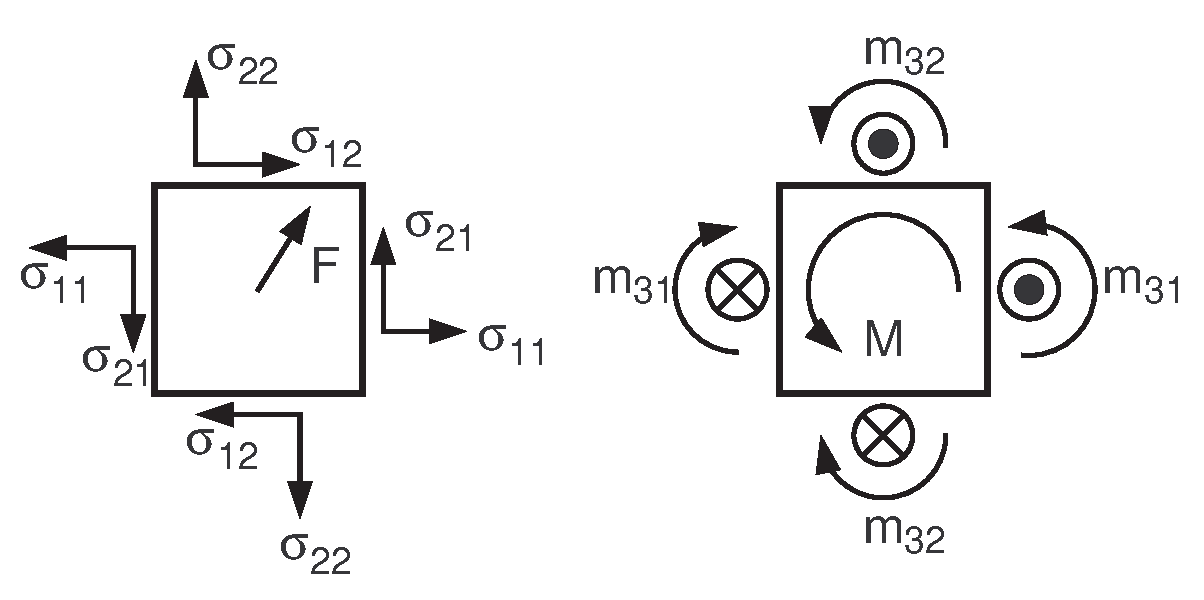
\includegraphics[width=0.8\textwidth]{inf_cosserat.eps}
\caption{The infinitesimal area element in 2D Cosserat elasticity.
  In addition to the standard situation, shown on the left, moments
  are applied to the area element.  $M$ is a moment/unit area (or
  moment/unit volume in 3D), and $m$ are moments/unit length (or
  moments/unit area in 3D).  The filled-in-dot or crossed-dot
  is the standard pictorial method for representing a moment ``coming
  out of or into the paper (respectively)'' using the right-hand screw
  convention.}
\label{inf_cosserat.fig}
\end{center}
\end{figure}

The micro-moments, $M$, are considered to produce micro-rotations in
the material.  One can think of the material being made up of grains
which are stuck together with an elastic glue.  The positions and
orientations of the grains can be measured.

This is described mathematically as follows.  The centres of mass of
the grains move according to
$$
x \rightarrow x + u_{x} \mand y\rightarrow y+ u_{y} \ ,
$$
in the standard way.  This also rotates the grains relative to their
initial orientation through an angle
$$
\theta = \ha(\pl_{x}u_{y}-\pl_{y}u_{x}) \ .
$$
For example, in Figure~\ref{deformation_cosserat.fig}, the grains have
moved according to
\begin{equation}
\left(\begin{array}{c}x\\y\end{array}\right) \rightarrow
\left(\begin{array}{cc}\cos\theta & -\sin\theta \\ \sin\theta & \cos\theta
\end{array}\right)
\left(\begin{array}{c}x\\y\end{array}\right)
\approx
\left(\begin{array}{c}x - \theta y\\y + \theta x\end{array}\right)   \ .
\label{rigid.rot.eqn}
\end{equation}
(The approximation holds for small $\theta$.)  This has rotated the
grains through an angle of $\theta$ about the origin, and if standard
elasticity were being used, this would be the end of story.  However,
now suppose that the individual grains can additionally rotate without
deforming the surrounding continuum (called `glue' above), as also
depicted in Figure~\ref{deformation_cosserat.fig}.  Denote by
$\thetac$ the angle between the original orientation (before
deformation by ${\mathbf u}$), and the final orientation.  Then
$$
\thetarel = \thetac - \theta \ ,
$$
is the relative rotation between how the grains are actually oriented,
and how they would be oriented if only the deformation ${\mathbf u}$
had been used.

\begin{figure}[htb]
\begin{center}
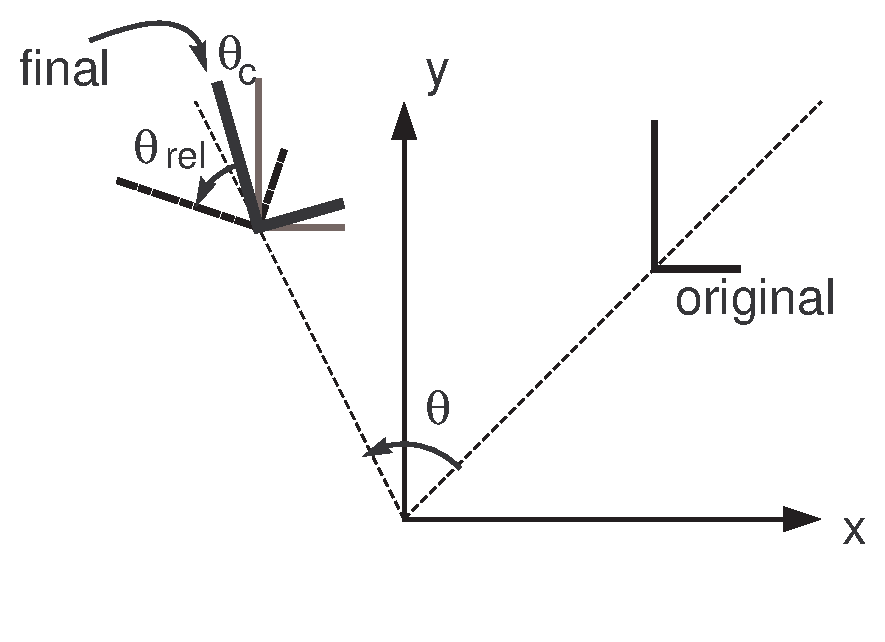
\includegraphics[width=0.6\textwidth]{deformation_cosserat.eps}
\caption{An original grain with orientation shown by the ``L''
  attached to it sits on the right.  This is deformed by ${\mathbf
  x}\rightarrow {\mathbf x}+{\mathbf u}$ and the result is shown by a
  dot-dashed ``L''.  In this case it is a simple rotation through
  $\theta>0$ (anticlockwise angles are positive).  The grain is then
  rotated through angle $\thetarel$, which in this case is negative, to
  the final bold-faced ``L'' orientation.  This final configuration is
  also obtained by deforming via ${\mathbf u}$ without any rotation of
  the ``L'' (resulting in the grey ``L''), and then rotating through
  an angle of $\thetac$ (positive in this case).}
\label{deformation_cosserat.fig}
\end{center}
\end{figure}

Natural measures of infinitesimal strain are
\begin{equation}
\left(\begin{array}{c}
\gamma_{xx} \\
\gamma_{yy} \\
\gamma_{yx} \\
\gamma_{xy} \\
\pl_{x}\thetac \\
\pl_{y}\thetac
\end{array}
\right) \equiv
\left(\begin{array}{c}
\pl_{x}u_{x} \\
\pl_{y}u_{y} \\
\pl_{x}u_{y}-\thetac \\
\pl_{y}u_{x}+\thetac \\
\pl_{x}\thetac \\
\pl_{y}\thetac
\end{array}
\right) =
\left(\begin{array}{c}
\ep_{xx} \\
\ep_{yy} \\
\ep_{xy}-\thetarel \\
\ep_{xy}+\thetarel \\
\pl_{x}\thetac \\
\pl_{y}\thetac
\end{array}
\right)
\label{nat.2d.deform.measures}
\end{equation}
These are natural for the following reasons.  Importantly, these
measures transform covariantly under both
$x\rightarrow -x$ and $y\rightarrow -y$.    This is
because under each of these $\thetarel\rightarrow -\thetarel$, which may be
understood from a number of different perspectives, such as handedness
change under these transformations.  Hence the quantity $\ga_{ij}$
transfoms naturally.  Moreover, performing a rigid rotation of the
material (see Eq.~(\ref{rigid.rot.eqn})) gives
$$
u_{x}=-\theta y \ , \spa
u_{y}=\theta x \ , \spa
\thetarel = 0 \ , \spa
\thetac = \theta \ ,
$$
which leaves $\ga_{ij}$ invariant.  This is important, as such a rigid
transformation should not cost any energy (it is simply a change of
reference frame).  This is why, for instance $\pl_{y}u_{x}+\thetac$ is
more natural than $\pl_{y}u_{x}+\thetarel$.



\chapter{Cosserat elasticity in 3D}
\label{3d.coss.elas.gen.sec}

The author would like to thank Ioannis Stefanou (ENPC, France) for his
help in writing parts of this Chapter.

Consider an infinitesimal 3D volume element with body force per unit
volume $\mathbf{F}$ and moment per unit volume $\mathbf{M}$.  Denote
the stress tensor by $\si_{ij}$ and the couple-stress pseudo tensor by
$m_{ij}$, so that the force density and moment density acting on a
surface with outward normal $\mathbf{n}$ are
$$
\mbox{force density}_{i} = \si_{ij}n_{j} \mand
\mbox{moment density}_{i} = m_{ij}n_{j} \ ,
$$
respectively.  The situation is shown graphically in 2D in
Figure~\ref{inf_cosserat.fig} and the 3D extension is obvious.
Equilibrium of the volume $V$ is equivalent to requiring
\begin{eqnarray*}
0 & = & -\int_{V}\rho \ddot{x}_{i} + \int_{\pl V}\si_{ij}n_{j} +
\int_{V}F_{i} \ , \\
0 & = & -\int_{V}\rho \ep_{ijk}x_{j}\ddot{x}_{k} + \tilde{\rho}\ddot{\theta}_{c} =
\int_{\pl V}\left(\ep_{ijk}x_{j}\si_{kl}n_{l} + m_{ij}n_{j}\right) +
\int_{V}\left(\ep_{ijk}x_{j}F_{k} + M_{i}\right) \ .
\end{eqnarray*}
These are standard equations, save for the inclusion of $\tilde{\rho}$
which parameterises the inertial effects of rotating, $m_{ij}$ and
$M_{i}$, and by using the divergence theorem and the arbitrary nature
of $V$, the following equations of equilibrium are obtained:
\begin{eqnarray}
0 & = & \nabla_{j}\si_{ij} + F_{i} \ , \non \\
0 & = & \nabla_{j}m_{ij} - \ep_{ijk}\si_{jk} + M_{i} \ .
\label{eqns.equjilb}
\end{eqnarray}

\section{Principal of virtual work and deformations}
\label{pov.sec}

Propose that the stress and couple stress are conjugate to
displacements $u_{i}$ and rotations $\thetac_{i}$ (which are kinematically
independent) through the following principal of virtual work
$$
\int_{\pl V}\left(\de u_{i}\si_{ij}n_{j} + \de\thetac_{i} m_{ij}n_{j}\right) +
\int_{V}\left(\de u_{i}F_{i} + \de\thetac_{i} M_{i}\right) = \int_{V}\de\mathcal{E} \ ,
$$
where $\mathcal{E}$ is a small change in the potential energy of the
medium, and $\de u_{i}$ and $\de\thetac_{i}$ are virtual displacements and
rotations of the medium's particles.  Using the divergence theorem,
the arbitrary nature of $V$ and the equation of force equilibrium
results in
$$
\de\mathcal{E} = \si_{ij}\left(\nabla_{j}u_{i}+\ep_{ijk}\de\thetac_{k}\right) +
m_{ij}\nabla_{j}\de\thetac_{i} = \si_{ij}\de\ga_{ij} + m_{ij}\de\ka_{ij}
\ ,
$$
where
\begin{equation}
\ga_{ij} = \nabla_{j}u_{i} + \ep_{ijk}\thetac_{k} \mand
\ka_{ij} = \nabla_{j}\thetac_{i} \ .
\label{ga.and.om.defns}
\end{equation}
Hence, the energy density is a function of $\ga_{ij}$ and $\ka_{ij}$:
$$
\mathcal{E} = \mathcal{E}(\ga_{ij},\ka_{ij}) \ ,
$$
with variation of the energy resulting in
$$
\si_{ij} = \frac{\pl \mathcal{E}}{\pl \ga_{ij}} \mand
m_{ij} = \frac{\pl \mathcal{E}}{\pl \ka_{ij}} \ .
$$
The deformation measures given in Eq.~(\ref{nat.2d.deform.measures})
are evident.  For instance the antisymmetric part,
$$
\ga_{[12]}=\ha(\ga_{12}-\ga_{21}) =
\ha(\pl_{2}u_{1}-\pl_{1}u_{2})+\thetac_{3} \ .
$$
The form of $\ga_{ij}$ given in 2D was motivated through consideration
of covariance under certain coordinate transformations, while here its
form appears through the `natural' proposition for the principal of
virtual work.

\section{Hooke's law for an isotropic material}

Since $\ga_{ij}$ is a proper tensor and $\ka_{ij}$ is a pseudo
vector, the most general second-order form for the energy density is
$$
\mathcal{E} = \mbox{$\frac{1}{4}$}\la(\tr\ga)^{2} +
\mu\ga_{(ij)}\ga_{(ij)} - \al\ga_{[ij]}\ga_{[ij]}
+ \mbox{$\frac{1}{4}$}\be(\tr\ka)^{2} +
\ga\ka_{(ij)}\ka_{(ij)} - \ep\ka_{[ij]}\ka_{[ij]}  \ .
$$
Round brackets indicate symmetric parts while square brackets indicate
antisymmetric parts: $\ga_{(ij)} = \ha(\ga_{ij}+\ga_{ji})$ and
$\ga_{[ij]}=\ha(\ga_{ij}-\ga_{ji})$.  The notation for the moduli is
chosen so that $\la$ and $\mu$ are the usual Lame constants, and I
hope that in the following formulae, the modulus $\ga$ can be
distinguished from the deformation measure $\ga_{ij}$.  The moduli
$\al$, $\be$, $\ga$ and $\ep$ are used in this section {\em only}.

Varying the energy gives
\begin{eqnarray}
\si_{ij} & = & \la\de_{ij}\tr\ga + 2\mu\ga_{(ij)} + 2\al\ga_{[ij]} \ ,
\non \\
m_{ij} & = & \be\de_{ij}\tr\ka + 2\ga\ka_{(ij)} + 2\ep\ka_{[ij]} \ .
\label{eqn.stress.couple.stress.3d.}
\end{eqnarray}
The equations for Cosserat elasticity for an isotropic medium are
Eqs.~(\ref{eqns.equjilb}), (\ref{ga.and.om.defns})
and~(\ref{eqn.stress.couple.stress.3d.}).  At each point on the
boundary of the material the surface loads and couples, or the
displacements and rotations must be specified.

The static equations in terms of $u$ and $\thetac$ are
\begin{eqnarray*}
0 & = & (\la+2\mu)\nabla(\nabla\cd u) -
(\mu+\al)\nabla\times(\nabla\times u) + 2\al\nabla\times\thetac + F
\ , \\
0 & = & (\be+2\ga)\nabla(\nabla\cd\thetac) -
(\ga+\ep)\nabla\times(\nabla\times\thetac) + 2\al\nabla\times u -
4\al\thetac + M \ .
\end{eqnarray*}


%%%
\chapter{3D layered Cosserat elasticity}
%%%

Layered Cosserat elasticity is a generalisation of standard
(non-Cosserat) transversely-isotropic elasticity.  The theory
considers the situation where the medium is comprised of a stack of
flat layers perpendicular to the $z$ direction.  The layers have
thickness $h$ and are separated from each other by an interface
material.  The interface material has thickness $h_{\mathrm{i}}$,
Young's modulus $E_{\mathrm{i}}$ and shear modulus $G_{\mathrm{i}}$.
The theory describes the limit
\begin{equation}
h_{\mathrm{i}} \rightarrow 0 \ , \ \ \
E_{\mathrm{i}} \rightarrow 0 \ , \ \ \
E_{\mathrm{i}}/h_{\mathrm{i}} \rightarrow hk_{n} \ \ \ \mbox{and}
\ \ \
G_{\mathrm{i}}/h_{\mathrm{i}} \rightarrow hk_{s} \ .
\label{thin.layer.limits.eqn}
\end{equation}
Here $k_{n}$ is called the normal stiffness, and $k_{s}$ is the shear
stiffness.  As will become more obvious below, the fact that
$E_{\mathrm{i}}/h_{\mathrm{i}}$ depends on $h$ is natural, since the
thicker the layers, the less important the macroscopic effect on the
thin interface.  The Cosserat rotation around $z$, $\thetac_{z}=0$ by
definition.

In this situation, the equations
are Eqs.~(\ref{eqns.equjilb}), (\ref{ga.and.om.defns}), the a-priori
definition $\thetac_{z}=0$, and the
consitutive relationships
\begin{eqnarray}
\sigma_{ij} & = & E_{ijkl}\gamma_{ij} \ , \\
m_{ij} & = & B_{ijkl}\kappa_{ij} \ .
\end{eqnarray}
$E$ is called the elasticity tensor, and $B$ is the bending rigidity
tensor, and are written below in terms of the layer Young's modulus
$E$, Poisson ratio $\nu$, and the parameters $h$, $k_{n}$ and $k_{s}$.

$E$ and $B$ may be derived by taking the
Equation~(\ref{thin.layer.limits.eqn}) limits of standard equations.
For instance, a layered material consisting of homogeneous, isotropic
layers in volume ratios $\alpha$ (for the ``main'', ``thick'' layers),
and $\alpha_{\mathrm{i}}$ (for the interface layers)
\begin{eqnarray}
E_{xxxx} & = & \alpha E_{xxxx}^{\mathrm{main}} + \alpha_{\mathrm{i}}E_{xxxx}^{\mathrm{i}} -
\alpha\alpha_{\mathrm{i}} \frac{ \left(
  \frac{\nu}{1-\nu}E_{xxxx}^{\mathrm{main}} - \frac{\nu_{\mathrm{i}}}{1 -
    \nu_{\mathrm{i}}}E_{xxxx}^{\mathrm{i}} \right)^{2}
}{E_{xxxx}^{\mathrm{main}}E_{xxxx}^{\mathrm{i}}} E_{zzzz} \ , \\
E_{xxzz} & = & \left( \alpha \frac{\nu}{1-\nu} +
\alpha^{\mathrm{i}}\frac{\nu^{\mathrm{i}}}{1-\nu^{\mathrm{i}}} \right) E_{zzzz} \ , \\
E_{zzzz} & = & \left( \frac{\alpha}{E_{xxxx}^{\mathrm{main}}} +
\frac{\alpha^{\mathrm{i}}}{E_{xxxx}^{\mathrm{i}}} \right)^{-1} \ .
\end{eqnarray}
Here
\begin{equation}
E_{xxxx}^{\mathrm{main}} = E\frac{1-\nu}{(1 + \nu)(1 - 2\nu)} \ ,
\end{equation}
which is a standard equation from non-Cosserat elasticity written in
terms of the ``main'' layers' Young's modulus $E$ and Poisson's
ratio $\nu$.  Substituting $\alpha = 1$, $\alpha_{\mathrm{i}} =
h_{\mathrm{i}}/(h + h_{\mathrm{i}})$, and taking the limits of
Equation~(\ref{thin.layer.limits.eqn}), yields
\begin{eqnarray}
E_{0000} = E_{1111} & = & \frac{E}{1 - \nu^{2} -
  \frac{\nu^{2}(1+\nu)^{2}}{1 - \nu^{2} + E/(hk_{n})}} \ , \nonumber
\\
E_{0011} = E_{1100} & = & \frac{\nu}{1-\nu}E_{0000} \ , \nonumber \\
E_{2222} & = & \left( \frac{(1+\nu)(1-2\nu)}{(1-\nu)E} +
\frac{1}{hk_{n}} \right)^{-1} \ , \nonumber \\
E_{0022} = E_{1122} = E_{2200} = E_{2211} & = &
\frac{\nu}{1-\nu}E_{2222} \ .
\end{eqnarray}
The shear terms may be motivated in a similar way, and are defined in
terms of the shear modulus of the ``main'' layers, $G$, and the
modified shear, $\tilde{G}$:
\begin{equation}
G = \frac{E}{2(1+\nu)} \ \ \ \mbox{and}\ \ \ \tilde{G} = \left(
\frac{1}{G} + \frac{1}{hk_{s}} \right)^{-1}
\end{equation}
They
are\footnote{Some references are the following.  DP Adhikary, HB Muhlhaus, AV
  Dyskin ``A numerical study of flexural buckling of foliated rock
  slopes'' International Journal for Numerical and Analytical Methods
  in Geomechanics 25 (2001) 871--884.  DP Adhikary, HB Muhlhaus, AV
  Dyskin ``Modelling the large deformations in stratified media ---
  the Cosserat continuum approach'' Mechanics of Cohesive-Frictional
  Materials 4 (1999) 195--213.}
\begin{eqnarray}
E_{0101} = E_{0110} = E_{1001} = E_{1010} & = & G \ , \nonumber
\\
E_{0202} = E_{0220} = E_{2002} = E_{1212} = E_{1221} = E_{2112} & =
& \tilde{G} \ , \nonumber \\
E_{2020} = E_{2121} & = & \mbox{$\frac{1}{2}$}(G + \tilde{G})\ .
\label{eqn.shearE.layered}
\end{eqnarray}
These are the only nonzero components of $E$.

The last equality of Equation~(\ref{eqn.shearE.layered}) implies that
$E$ does not obey the usual symmetries, ie $E_{ijkl}\neq E_{jikl}$, as
should be expected in the Cosserat situation.
Equations~(\ref{eqn.shearE.layered}) are easily motivated.  Firstly,
any shear in the $(x,y)$ plane should behave independently of the
layers, which motivates the first equation.  Now consider the case
$k_{s}=0$: that is, the Cosserat layers may slide freely over one
another ($\tilde{G}=0$).  Shear strains $\gamma_{02}$ or $\gamma_{12}$
involves layers sliding over one another.  For instance, $u_{0} =
x_{2}$ gives $\gamma_{02}=1$.  This should cost zero energy, which is
encoded in $E_{ij02}=\tilde{G}=E_{ij01}$.  However, a nonzero shear
strain $\gamma_{20}$ or $\gamma_{21}$ involves shearing the ``main''
layers, resulting in the last equality of
Equations~(\ref{eqn.shearE.layered}).

Finally, the only nonzero components of $B$ are defined in terms of
the bending rigidity of a layer
\begin{equation}
D = \frac{Eh^{3}}{12(1-\nu^{2})} \ ,
\end{equation}
and are
\begin{eqnarray}
B_{0101} = B_{1010} & = & \frac{D}{h} \left(\frac{G - \tilde{G}}{G +
  \tilde{G}}\right) \ , \nonumber \\
B_{0110} = B_{1001} & = & -\nu B_{0101} \ .
\end{eqnarray}
The negative sign in the last equation is not a typo~\footnote{See, for
  instance the following.  R Lakes ``Experimental methods for study of
  Cosserat elasticity solids and other generalised elastic continua'',
  Equation (4) and discussion following Equation (18).  S Forest
  ``Mechanics of Cosserat media: An introduction'' Equation (A50) and
  discussion of (B65)}.




\end{document}

